%% PNAStwoS.tex
%% Sample file to use for PNAS articles prepared in LaTeX
%% For two column PNAS articles
%% Version1: Apr 15, 2008
%% Version2: Oct 04, 2013

%% BASIC CLASS FILE
\documentclass{pnastwo}

%% ADDITIONAL OPTIONAL STYLE FILES Font specification

%\usepackage{pnastwoF}
%\usepackage{cite}
\usepackage[numbers,round,sort,compress]{natbib}
\bibpunct{(}{)}{,}{n}{,}{,}  % https://xianblog.wordpress.com/tag/natbib/ (allows natbib with PNAS)
\usepackage{lineno}
\setlength\linenumbersep{2pt}
\usepackage{placeins}
\usepackage{float}

%% OPTIONAL MACRO DEFINITIONS
\def\s{\sigma}
%%%%%%%%%%%%
%% For PNAS Only:
\url{www.pnas.org/cgi/doi/10.1073/pnas.0709640104}
\copyrightyear{2008}
\issuedate{Issue Date}
\volume{Volume}
\issuenumber{Issue Number}
%\setcounter{page}{2687} %Set page number here if desired
%%%%%%%%%%%%

\begin{document}

\title{The Impact of Bias in Landcover Maps}
%\title{Our Understanding of Global Change is Built on a Shaky Foundation}

\author{Lyndon Estes\affil{1}{Princeton University, Princeton, NJ USA},
Peng Chen\affil{2}{Indiana University, Bloomington, IN USA},
Stephanie Debats\affil{1}{Princeton University, Princeton, NJ USA},
Tom Evans\affil{2}{Indiana University, Bloomington, IN USA},
Fanie Ferreira\affil{3}{GeoTerraImage, Pretoria, RSA},
Gabrielle Ragazzo\affil{1}{Princeton University, Princeton, NJ USA},
Justin Sheffield\affil{1}{Princeton University, Princeton, NJ USA}
Adam Wolf\affil{1}{Princeton University, Princeton, NJ USA}
\and
Kelly Caylor\affil{1}{Princeton University, Princeton, NJ USA}}

\contributor{Submitted to Proceedings of the National Academy of Sciences
of the United States of America}

%%%Newly updated.
%%% If significance statement need, then can use the below command otherwise just delete it.
%\significancetext{LDE developed the concept of the study, conducted the analysis, data interpretation and drafted the manuscript. \color{red}{To be completed}}

\maketitle

\begin{article}
\begin{abstract}
{Blah blah.}
\end{abstract}

\keywords{landcover | bias | remote sensing | agriculture | crop yield | harvested area | carbon | agent-based model | landscape}

\abbreviations{GTI, GeoTerraImage; SSA, sub-Saharan Africa}
\linenumbers

\dropcap{T}he nature and distribution of landcover is an indicator that gives significant insight into socio-econonomic processes \cite{lambin_modelling_1997}, because human endeavors are so closely tied to how we transform land, whether it be the felling of ancient forests for farmland or erecting skycrapers. The vastness of our alteration of Earth�s landscapes suggests that landcover is a fundamental mediator of many environmental and social processes that drive or are affected by global change \cite{lambin_modelling_1997}, such as agricultural production and food security \cite{lark_cropland_2015,wright_recent_2013, licker_mind_2010}, carbon cycling \cite{asner_high-resolution_2010,gaveau_major_2014}, biodiversity loss \cite{newbold_global_2015,luoto_predicting_2004}, and changes in human demography \cite{linard_assessing_2010}. Like any view into nature, resolution and fidelity at fine scales are the keys to unlocking more granular and mechanistic insights into these processes \cite{see_improved_2015}. It is therefore unsurprising to see the explosive growth in private sector initiatives to develop new Earth observing capabilities, which range from small hobbyist drones\footnote{e.g. 3DRobotics, DJIA} to satellite arrays\footnote{Planet Labs, Skybox}, in order to add value to industries such as agriculture, mining, and construction. This rapid growth in fine-scale landcover mapping capability is creating new opportunities to develop actionable information for traditionally public-sector concerns, such as agricultural development\footnote{USAID's Feed the Future}, drought and flood adaptation\footnote{Global Index Insurance Facility, www.indexinsuranceforum.org}, and carbon cycle management\footnote{United Nations REDD+, www.un-redd.org/aboutredd}. But while the demand for more nuanced, landcover-based insights is growing, there is only now the opportunity to use finer-scaled imagery to comprehensively interrogate the accuracy and biases in the landcover products that have become ubiquitous in global change research.

Global landcover data can only practically be derived from satellite imaging, but in many regions the average size class of the cover type of interest is smaller than the sensor resolution, or spectrally indistinct from other neighboring covers, which propagates classification error \cite{see_improved_2015,lobell_use_2013,estes_diylandcover:_2015}. The result is that landcover maps are generally inaccurate at finer scales and disagree greatly, particularly in those parts of the world undergoing the most rapid land use changes, where these sources of bias tend to be most pronounced \cite{estes_projected_2013,fritz_comparison_2010,fritz_cropland_2011}.  

Errors in landcover products are widely-acknowledged \cite{fritz_comparison_2010, fritz_cropland_2011, see_improved_2015, fritz_mapping_2015,verburg_challenges_2011}, and there are a variety of efforts underway to improve landcover maps, particularly for agriculture \cite{fritz_geo-wiki:_2012,estes_diylandcover:_2015}. What is less known is the degree to which these errors bias analyses derived from the distributional and areal information in landcover. Errors are hard to quantify because spatially extensive reference data are not available for most regions of the world--particularly over Africa and other developing regions. Error assessments therefore typically rely on a small number of ground truth points for a bottom-up assessment or aggregated survey data for a top-down sanity check. For this reason, we have a better understanding of discrepancies between landcover datasets in relation to country-level statistics \cite{fritz_comparison_2010,fritz_cropland_2011,kaptue_tchuente_comparison_2011}, which offers little direction for how to arrive at a true number. 

Being unable to fully quantify the errors in landcover maps of course makes it difficult, if not impossible, to quantify their impact on downstream analyses. There has been some work examining how such error influences climate simulations \cite{ge_impacts_2007}, agricultural land use patterns \cite{schmit_limitations_2006}, and carbon flux \cite{quaife_impact_2008} and human population estimates \cite{linard_assessing_2010}, but these either use simulated landcover errors \cite{ge_impacts_2007} or compare relevant differences in estimates between different satellite-derived landcover maps \cite{linard_assessing_2010, quaife_impact_2008}. One exception is a study  \cite{schmit_limitations_2006} that used a high quality, ground-collected reference map detailing farm land use parcels in central Belgium, but the number of sites and region were both fairly restricted, and the parcels were not spatially contiguous. 

Just as a tall edifice cannot be built on a shaky foundation, global change science needs to be based on sound landcover data. There is thus an urgent need to more precisely quantify landcover map errors and how these vary over large regions, particularly for the regions where landcover is changing most rapidly yet is most poorly known.  We address this need in this study, using a unique, high accuracy agricultural landcover map for the entire country of South Africa to quantify the errors in several latest generation landcover maps that are widely used in global change studies.  We use this information to examine how i) landcover properties and related classification schemes influence error, ii) how these errors change with aggregation scale, with the specific goal of determining ``safe'' scales for drawing area-based inferences, and iii) how these errors propagate through several different forms of downstream analyses that broadly represent the global change research focus areas, including biogeochemical and land use change studies, food security assessments, land surface hydrology and climatology, and human geography.  

\vspace{-0.5 cm}
\section{Study area and landcover data}
South Africa comprises nearly 6\% of sub-Saharan Africa's (SSA) landmass, and has a large, diverse agricultural sector, ranging from large commercial operations to smallholder farms \cite{hardy_rainfed_2011,estes_using_2014}. This diversity suggests that the country's agricultural landcover spans the range of types that are found throughout the rest of SSA.  

The South African government commissioned a whole country cropland boundary map to enhance its annual collection of agricultural statistics \cite{fourie_better_2009}. The map was made by trained workers who visually interpreted high resolution satellite imagery ($<$5 m SPOT imagery) and manually digitized field boundaries following a standardized mapping protocol. The resulting vectorized field maps, which were made in 2007 and updated in 2011, provide a unique, high quality reference dataset describing crop field distributions and size classes, and are 97\% accurate in distinguishing cropland from non-cropland at 200 m resolution. We intersected the field vectors with a 1 km grid, and calculated the percent of each cell occupied by fields to create a gridded cropland reference map. 

We compared the reference map with similar maps derived from four existing landcover datasets. We obtained South Africa's 30 m resolution National Landcover map (SA-LC) for 2009 \cite{sanbi_national_2009}, the 500 m resolution MODIS Landcover for 2011 \cite{land_processes_distributed_active_archive_center_lp_daac_modis_2011, friedl_modis_2010}, the 300 m resolution GlobCover 2009 \cite{arino_global_2012}, and the new 1 km Geo-wiki hybrid-fusion cropland map for Africa \cite{fritz_mapping_2015}. We chose these particular datasets because they are nearly contemporaneous with our reference data, and represent the major types of landcover products used by researchers: SA-LC typifies the higher resolution, Landsat-derived maps that are developed individually for many countries \cite[e.g.][]{fry_completion_2009}, MODIS and GlobCover are widely used global-scale products \cite{gross_monitoring_2013,shackelford_conservation_2015}, while Geo-Wiki incorporates the first three datasets and represents the current state-of-the-art in landcover mapping. We extracted the cropland classes from the first three datasets and converted these to 1 km resolution percent cropland estimates (hereafter simply the ``cropland maps''), resulting in 4 maps to compare to our reference map.  

\vspace{-0.5 cm}
\section{Quantifying Error and Bias}
We first quantified the errors in cropland area estimates based on the pixel-wise differences between the reference map and each of the four cropland maps. We calculated these errors for five different scales of aggregation, from the original 1 km up to 100 km, in order to calculate bias--the average pixel-wise error--and how it varies with scale. Next, we assessed the degree to which the pattern of agricultural landscapes, expressed in terms of the mean cropland cover, impacts bias.    

We then investigated how these landcover map biases propagate through data that are built upon them. We began by examining the biases in three different kinds of landcover-based data that we consider to be ``first-order'', in that they are derived by mapping a variable of interest to a landcover type(s). The first of these was to assess potential biases in Tier-1 carbon accounting maps that we constructed from the cropland maps, following \cite{ruesch_new_2008}. The second was an assessment of gridded maize yields derived by disaggregating district-scale agricultural census data for both maize yield and harvested area \cite[following][]{monfreda_farming_2008,ramankutty_farming_2008}. We used these same data to calculate gridded maize production estimates, which we used to conduct the third first order analysis.   

Finally, we conducted two second-order analyses, in which a process model draws on the cover types' values to calculate an output value. For the first of these, we examined how cropland map biases influence 25 km resolution monthly evapotranspiration calculated by the Variable Infiltration Capacity \cite{liang_simple_1994} land surface hydrology model. For this example, we used the cropland maps to adjust landcover-specific leaf area index (LAI) values that VIC uses to partition water vapor fluxes into their evaporative and transpirative components. In the second example, we examined how these errors can impact the parameterization of an agent-based food security model \cite{chen_dependency_2013}. Spatially-explicit, agent-based models are frequently employed in land change science, and require an initialization step to assign landscape resources to model agents  \cite[e.g.][]{manson_agent-based_2007,evans_multi-scale_2004,kelley_relative_2011}. In this case, we used cropland maps to provide the model the location and abundance of cropland, which is used to  allocate an initial share of cropland to each farm household (agent) in the model.  

\vspace{-0.5 cm}
\section{Bias}
\subsection{Landcover bias}

We created the 1 km reference map after removing all field types classified as communal/smallholder agriculture (individual fields in this category were not mapped, thus they were removed to prevent potential cropland area overestimates) or permanent tree-crops (SI), and calculated the total cropland extent in the remaining area (1,081,000 km$^2$, or 90\% of South Africa). The 2011 reference map showed a cropland area of 104,310 km$^2$, which the SA-LC and GeoWiki maps overestimated by 26 and 5.8\%, respectively, and GlobCover and MODIS underestimated by 21 and 26.1\%.  

We then aggregated the reference and each cropland map to 5, 10, 25, 50, and 100 km resolutions, and subtracted the four landcover maps from the reference map at each scale of aggregation to assess patterns of differences (Fig. 1). Negative pixels here represent overestimation error, while positive values indicate underestimates.

\vspace{-0.25 cm}
\begin{figure}[ht]
\centerline{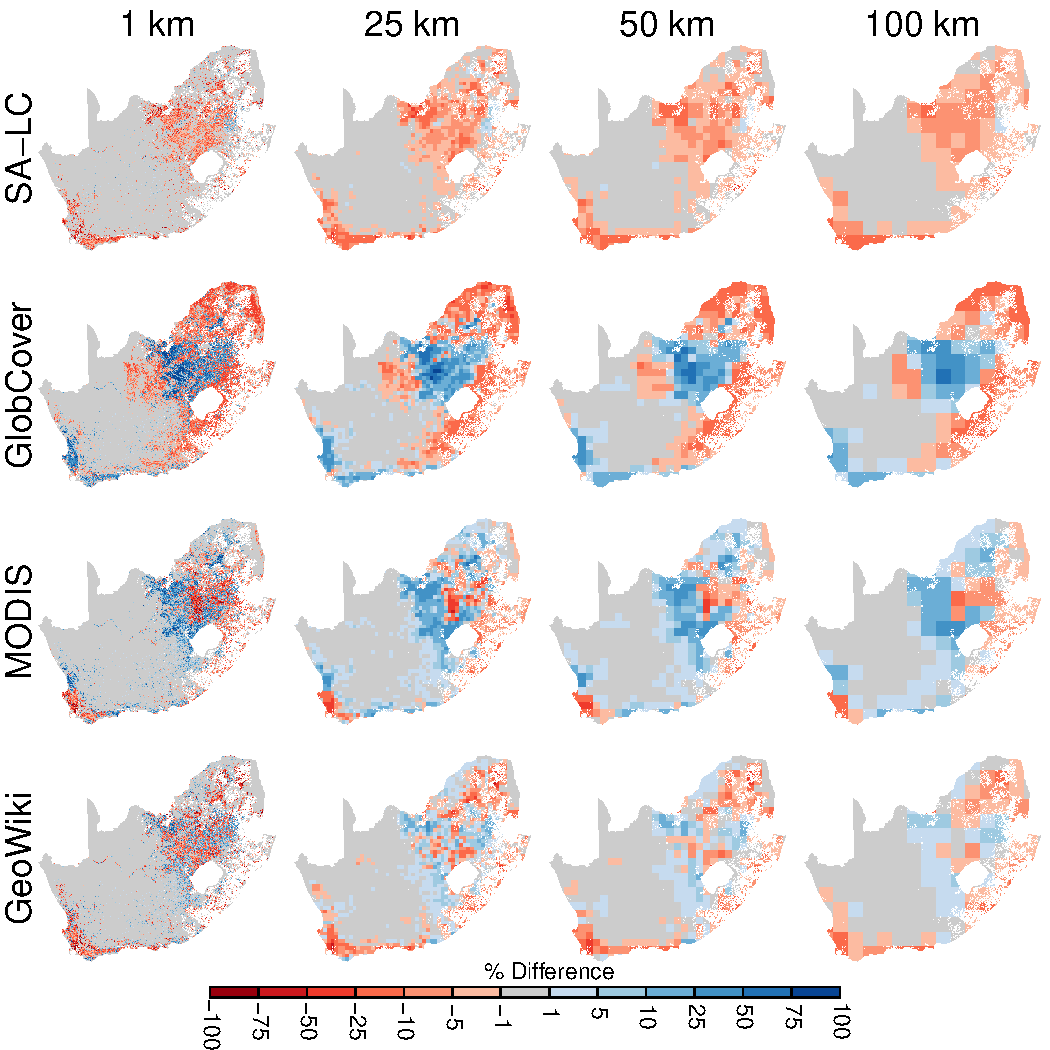
\includegraphics[width=.5\textwidth]{figures/bias_map.pdf}}
\caption{Differences in percent cropland estimates between the reference map and each of the four landcover maps. Rows indicate the landcover map being assessed (by subtraction from the reference map), while columns refer to resolution of aggregation. White indicates areas with no data where communal farmlands or plantation forests were removed.}\label{afoto}
\end{figure}

The most pronounced differences were in the MODIS and GlobCover maps, which both underestimated cropland extent by 10-75\% in the center of the country (blue areas in Fig. 1, and the dominant production region), and overestimated along the eastern to northern margins (red areas in Fig. 1). The differences between the reference and these two maps at 1 km resolution were respectively 21\% (MODIS) and 34\% (GlobCover), on average. This mean pixel-wise error expresses the amount of \emph{bias} in a map, that is its tendency to err in a particular direction. For MODIS, bias drops to 8\% at 50 km of aggregation, whereas GlobCover bias is 24\% at 100 km (SI Appendix, Fig. S1). 

The SA-LC map uniformly overestimated cropland throughout the country (Fig. 1), but was less biased, ranging from -8\% at 1 km to -6\% at 100 km  (Fig. S1). The GeoWiki map has a strongly heterogenous pattern of differences (Fig. 1) and the smallest magnitude of bias, which changed between slight tendencies to underestimate (5\% at 1 km) and overestimate (-2 \% at 100 km,  Fig. S1).    

\subsection{The role of landscape characteristics in shaping bias}
To investigate the degree to which landscape features influence landcover map bias, we extracted all pixels in agricultural areas ($>$0\% cropland) of the 1 km reference map using the boundaries of 354 magisterial districts (South Africa's finest administrative unit, which average 3,445 km$^2$ in size; SI Appendix, Fig. S3), and calculated the district-wise mean for these pixels to provide a measure of cropland density, and information on the degree of mixing between cropland and other land covers. We then extracted the cropland map errors for the same pixels, and calculated the absolute value of bias for each district. Absolute bias describes the magnitude of bias but not its direction, and is more informative about the likelihood of the map being biased at any given point in the landscape than actual bias, as positive and negative biases can cancel each other out within small areas. 

A generalized additive model fit to district-level absolute bias (log-transformed) shows that absolute bias peaks at 50\% cropland cover for all but the GlobCover map (which continued to increase with cropland cover), and is lowest when the landscape is dominated either by cropland or other cover types (Fig. 2). In other words, bias is highest when cropland cover is mixed evenly with other cover types. 

%\vspace{-1 cm}
\begin{figure}[ht]
\centerline{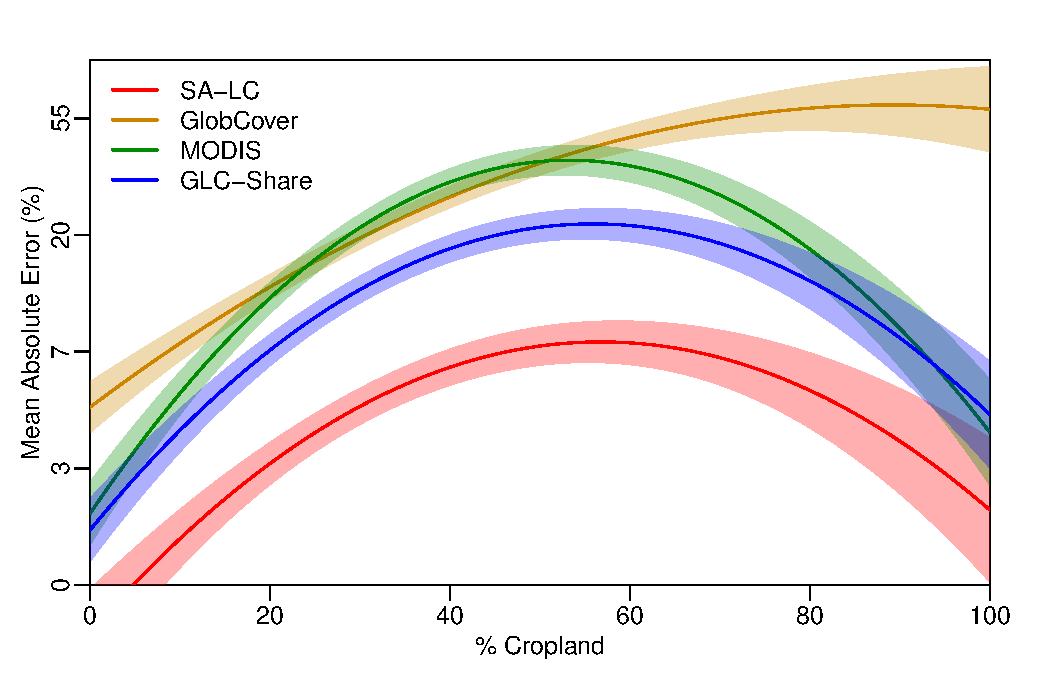
\includegraphics[width=.4\textwidth]{figures/biases_md_lnorm_gam_mu0.pdf}}
\caption{The relationship between the mean absolute bias in cropland maps and cropland cover within agricultural areas (reference map pixels having $>$0.5\% cropland), averaged within the boundaries of magisterial districts (n = 345), as fit with a generalized additive model. Prediction curves are color-coded to the different cropland maps, with the solid line indicating  predicted absolute bias, and the lighter shading the standard error of the coefficients. Models were also fit to the mean absolute biases across all four maps (black curve), and from all maps exlcuding GlobCover (grey surve).}
\label{afoto}
\end{figure}

\subsection{The impact of bias on calculating carbon stocks}
We used the data of \cite{ruesch_new_2008} to calculate carbon densities for African forests, shrublands, croplands, grasslands, and sparse habitats (semi-arid grasslands and low shrublands), assigning cropland carbon values to map cells in proportion to their cropland cover. For the non-cropland proportions, we assigned the carbon value from each of the other types, such that we created four different carbon maps for each landcover map at each aggregation scale (Fig. S4), which allowed us to test how carbon estimates vary as a function of i) cropland map bias and ii) the characteristics of adjacent cover types. 

The difference between total carbon stocks for the country made using any of the cropland maps were within +/-3\% of those based on the reference map, regardless of which cover type was adjacent to cropland (Table S1), because the large of non-cropland in the country ($\sim$50-70\%, Fig. 1) dilutes any map errors. Comparing total stocks between maps for just the agricultural area (30-50\% of the country) reveals much greater differences (Table S1). SA-LC overestimated carbon stocks by just 2\% when the adjacent cover type was forest, and up to 15\% when it was sparse cover. MODIS ranged from negligible differences in denser carbon classes (forest, secondary forest, and shrublands) to 8-13\% underestimates for the grassland and sparse classes. GeoWiki underestimated for all types, from $<$1\% for sparse cover to 8\% for forest. GlobCover grossly overestimated total carbon stocks for agricultural areas, varying from 64\% for sparse lands to 162\% for forest. The magnitude of this bias was due to false positives--GlobCover identified cropland in nearly 50\% of pixels, compared to 30\% for the other three cropland maps. 

The spatial patterns of errors in carbon estimates (Fig. S4) reflect those of cropland biases (Fig. 1). Where cropland was underestimated and the surrounding cover type was of higher carbon density than cropland, carbon density was overestimated. For lower density cover (grassland and sparse vegetation), carbon stocks were underestimated, but by small magnitudes. These tendencies were reflected in each map's biases, calculated over agricultural areas (Fig. 3). For example, MODIS and GlobCover bias was $\sim$-50\% (overestimation) at 1 km resolution when forest was the cropland-adjacent cover (stars in semi-transparent green and gold bars, Fig. 3; Table S2). For sparse vegetation (open circles in Fig. 3), MODIS bias was 3\% at all scales, whereas maps that overestimated cropland (e.g. SA-LC, semi-transparent red) overestimated carbon density for this cover type, because cropland has a higher carbon density \cite{ruesch_new_2008}. Overall, GeoWiki had the lowest bias, for all cover types and all resolutions. It worst bias was a tendency to overestimate by 12\% at 1 km when forest was adjacent, but at coarser scales this bias reduced to just a few percent (Fig. 3, Table S2). All maps' biases are within +/-10\% bias after aggregation to 25 km.

%\vspace{-0.9 cm}
\begin{figure}[!ht]
\centerline{\includegraphics[width=.4\textwidth]{figures/carbon_veg_scale3.pdf}}
\caption{The biases in carbon density estimates based on cropland maps, expressed as a percent difference relative to the reference map. The values of actual bias (incorporating bias direction and magnitude) and absolute bias (magnitude only) are presented in semi-transparent and solid colors, respectively, with colors denoting the specific cropland map and symbols indicating which cover type was used to calculate cropland adjacent carbon density. The bar represents the mean biases calculated across each of the 5 cover types. Shrubland and grassland bias values are near zero and not shown for display clarity.}
\label{afoto}
\end{figure}

Absolute bias in carbon maps (solid colored bars in Fig. 3) generally followed the same patterns, but with somewhat higher magnitudes and a few important differences. The most notable is that Geo-Wiki had fairly large absolute bias at 1 km, averaging 27\% across across cover types (line in solid blue bar, Fig. 3, Table S2), which is close to the 36-37\% for GlobCover and MODIS. SA-LC had the lowest absolute bias across scales, averaging (across cover types) from 14\% at 1 km to 3\% at 100 km. (Fig. 3, Table S2). The increase in Geo-Wiki's absolute bias relative to SA-LC's can be attributed to the highly heterogeneous nature of its cropland errors (Fig. 1), which varied between positive and negative over much shorter distances than the other three cropland maps.

\subsection{Bias in harvested areas, yield, and production estimates}
The disaggregated yield and harvested area maps of \cite{monfreda_farming_2008} are built upon cropland fraction maps where the total area is adjusted to match survey-derived agricultural area statistics reported for administrative districts \cite[provinces, in South Africa's case][]{ramankutty_farming_2008}. To be consistent with this methodology, we adjusted our cropland maps using the same procedure, but we used the reference map to calculate total cropland area for each of South Africa's nine provinces, and then updated the pixel-wise cropland percentages in the four cropland maps so that the province-wise sums matched the reference areas \cite[][and see SI]{ramankutty_farming_2008}. Despite this statistical constraint, the updated cropland maps still had large spatial errors that were similar in pattern (Fig. S5) to those in the unadjusted maps (Fig. 1), and we evaluated how these residuals affected gridded estimates of the yield and production of maize, South Africa's largest crop \cite{estes_comparing_2013}. To create these maps, we followed \cite{monfreda_farming_2008} by disaggregating district-level (n = 354, mean area = 3,445 km$^2$) agricultural census data \cite{statistics_south_africa_commercial_2007} for maize yield and harvested area, aggregated each set of maps, and multiplied the two to calculate production at each scale. 

The yields disaggregated onto the cropland maps were markedly different to those on the reference map, particularly in the lower density cropland areas in the center of the country, where GlobCover overestimated yields and MODIS and GeoWiki (to a lesser extent) underestimated them at 1 km resolution (Fig. S6). However, only GlobCover showed a notable bias in yields at this resolution, which was equivalent to nearly 60\% of the mean reference yield of 3.4 tons ha$^{-1}$. All other maps had biases of just +/-5\% at 1 km (Fig. 5). Interestingly, GeoWiki and MODIS biases increased with aggregation, peaking at 10 km where both had underestimation biases of 30\%, thereafter declining to 10\% at 100 km. In contrast, GlobCover's yield bias declined linearly with aggregation (Fig. 5). 

%\vspace{-1 cm}
\begin{figure}[ht]
\centerline{\includegraphics[width=.4\textwidth]{figures/yield_bias_scale.pdf}}
\caption{The biases in disaggregated maize yield and production estimates. The values of actual bias (incorporating bias direction and magnitude) and absolute bias (magnitude only) are presented in semi-transparent and solid colors, respectively, with colors denoting the specific cropland map and symbols indicating whether the bias is related to one of two yield aggregation methods and associated crop production estimates.}
\label{afoto}
\end{figure}

Production errors were completely unbiased (Fig. 5). The statistical constraints on harvested and cropland areas resulted in the canceling out of spatial errors in production estimates, which is evident in the checkerboard-like pattern in maps of production biases (Figure S7). However, this pattern of bias means that absolute bias in production estimates were large, between 40 to 55\% for GeoWiki, MODIS, and GlobCover at 1 km, and remained generally high (10-28\%) even up to 50 km of aggregation (Fig. 5). SA-LC production biases were lowest across all spatial scales (20\% at 1 km to 2\% in 100 km).  

Absolute mean biases in yield were also substantial, and generally 10-15\% larger than production biases across all spatial scales, except for GlobCover where absolute production biases exceeded yield bias at 5-100 km of aggregation. 

\subsection{Bias in evapotranspiration estimates}
Compared to carbon and crop related examples, actual and absolute biases in evapotranspiration calculated using the VIC model were small and averaged to less than +/-1\%. However, there are several hotspots of discrepancy evident in the error maps (Fig. 6). The most pronounced of these are the 5-15\% overestimates in the center of the country that resulted when VIC was initialized with MODIS and GlobCover, while overestimates along the southern and western coasts reached 25\%. These locations correspond primarily to the margins of major crop production regions--in the center is the westernmost boundary of the summer rainfall growing region, where maize is the primary crop, while the hotspot on the west coast marks the western boundary of the wheat-dominated winter rainfall region \cite{hardy_rainfed_2011}. These two boundaries respectively correspond to the 400 and 200 mm isohyets of growing season rainfall. 

SA-LC and GeoWiki also produced biased ET estimates along the southern and western coasts, but here the tendency was to underestimate ET, while biases in the center of the country were either negligible to absent.  All but MODIS underestimated ET by 5-15\% in the northern tip of the country.  

\FloatBarrier
\begin{figure}[ht]
\centerline{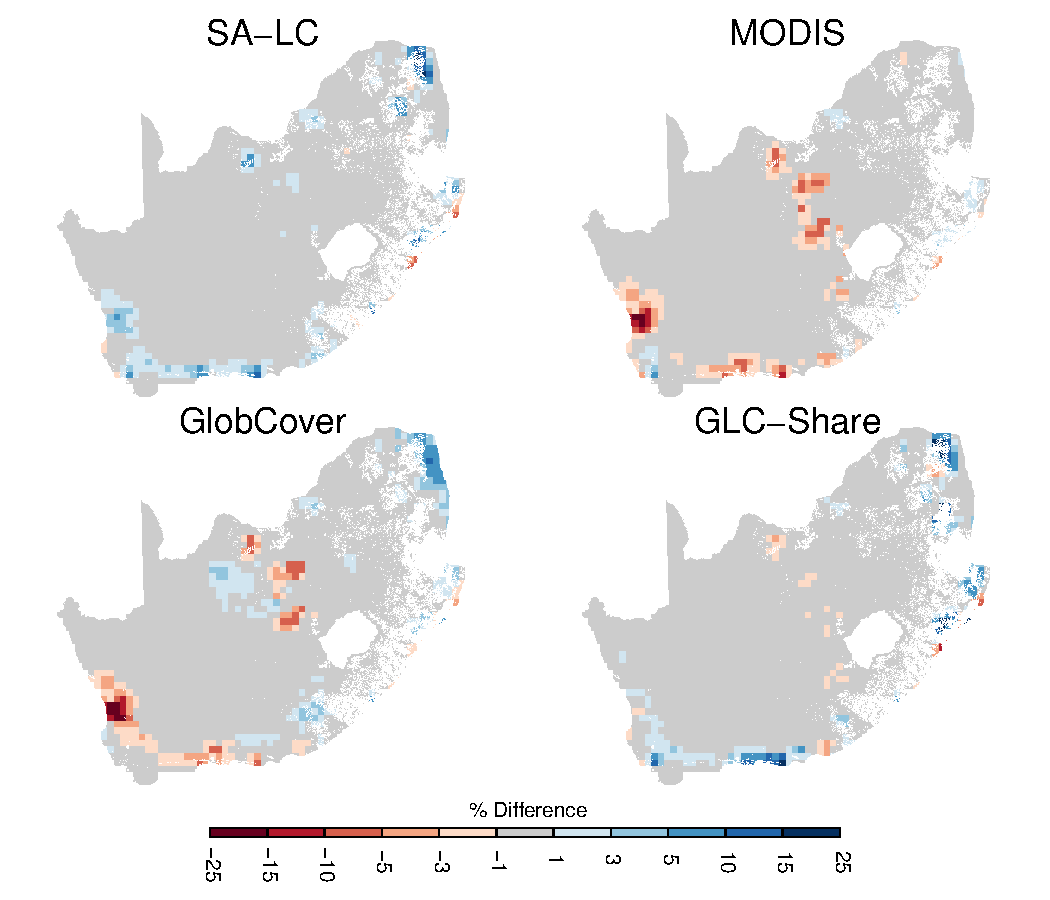
\includegraphics[width=.5\textwidth]{figures/et_bias_map.pdf}}
\caption{Differences in annual mean evapotranspiration estimates from 29-year runs of the VIC land surface hydrology model when initialized with LAI response curves derived from the reference map, versus those from the four cropland maps.}\label{afoto}
\end{figure}

\subsection{Initialization biases in agent-based models}
We used an agent-based model (ABM) of food security that represents the interactions between hundreds of individual farming households over multiple seasons \cite{chen_dependency_2013}. Like many spatial ABMs, the model is computationally intensive, and thus run over smaller geographic domains (e.g. districts, rather than an entire country) and at higher spatial resolutions (10s to 100s of meters) that are needed to represent the different land units of single farmers. To match these computational characteristics, we selected four contiguous magisterial districts (ranging from 1,040-1,343 km$^2$, Fig. S8) in the eastern part of the country, having between 28-45\% of their areas devoted to cropland, according to the reference map. 

We disaggregated the cropland percentages in all maps to binary cropland/non-cropland cover types with 100 m resolution, which matches the typical field size (1 ha) for smallholder farmers in household survey data (collected in Zambia) used in developing the agent-based model \cite{chen_dependency_2013}. These surveys found mean household crop field area to be 2 ha, which we divided into reference cropland areas to estimate the total households within each district. We then initialized the model by assigning each household agent two cropland pixels. In order to emulate the natural groupings of communities, the model only assigns a household fields that are within 1.5 km of other agents' fields, provided those pixels were not previously allocated to another agent. The model thus iteratively grows ``communities'' until all households are assigned cropland, or all available cropland is allocated. 

We used the reference map and each cropland map to separately initialize the model, and compared the agent allocation results to assess how cropland map errors impacted the initialization process. [insert importance here]. We examined two metrics, the first being the number of agents that were not assigned fields. Here there was a one-to-one relationship between the percentage of cropland area underestimation and the percentage of households left without farmland (Fig. 6, left panel). The most extreme examples occurred when MODIS cropland initialized the ABM in districts 1 and 2, where $\sim$85\% of agents did not receive cropland. 

All households were assigned fields when maps overestimated cropland extent (GeoWiki, SA-LC), but in these cases the percent of cropland left unallocated--our second metric for assessing cropland error impacts--matched the size of the overestimate (e.g. $\sim$20\% for SA-LC, Fig. 6 right panel). Interestingly, the overall relationship between the percent of cropland allocated and percent cropland error was U-shaped, as the model also failed to give land to households when cropland was underestimated by more than 50\% (Fig. 6, right panel). MODIS again provided the most pronounced results in districts 1 and 2, where 7-12\% of cropland was left unallocated despite the fact that 85\% of agents had no land. This curious relationship occurred because cropland tends to cluster, and when it is underestimated, the size of these clusters is small, resulting in islands of cropland that fall outside of the search radius (which is constrained by an absolute distance and the proximity of other agents) within which cropland is sought when agents are seeded onto the landscape. 

%randomly siting 100 household agents within each district, and allocating the nearest two cropland pixels to each household. The remaining agents are then iteratively assigned unallocated cropland pixels within a 1.5 km radius of existing agents' fields, and this process continues until all agents are assigned cropland, or all available cropland is allocated. This initialization process 

\begin{figure}[ht]
\centerline{\includegraphics[width=.5\textwidth]{figures/agent-bias.pdf}}
\caption{Biases in agent-based model initialization relative to the district-wise errors (as a percent) in total cropland area, measured in terms of the percent of households having no cropland allocated (left), and the percent of cropland left unallocated (right). Dot sizes correspond to district numbers, colors represent the landcover map.}
\label{afoto}
\end{figure}

\section{Discussion}

\begin{itemize}
  \item First large area quantification of spatial biases
  \item How large those biases are, for one of the most widely spread (spreading landcovers)
  \item Insight into causes of bias, and thus some understanding of where biases are likely to be greater or smaller
  \item How much progress made in reducing it
  \item Class type and bias
\end{itemize}


Some points to make thrown out now because out of time. Others will be added. Please add any important implications/considerations you see from the results.  

Some points from my notes last year: 
\begin{itemize}
  \item Bias as a function of scale
    \begin{enumerate}
      \item At 1 km resolution all landcover products are still fairly biased.  
       \item Bias drops to acceptable levels quickly for geowiki--at 5X5 km, mean bias is just 1\% (overestimated). The absolute bias for this dataset is 10\% or lower from 10X10 km resolution and coarser.  
       \item The SA dataset's bias is fairly consistent but low across all levels of aggregation, amounting to no more than an 8\% overestimate of cropland with absolute bias of similar magnitude. 
       \item MODIS and GlobCover biases (mostly of underestimation) do not dissipate until the higher levels of aggregation. MODIS's actual bias (under-estimation) falls below 10\% at 20 km resolution, but the absolute bias remains above 10\% until more than a 100-fold aggregation is done ($>$100 km resolution).  For GlobCover, it is still too high.  
    \end{enumerate}
  \item Bias as a function of cropland cover
    \begin{enumerate}
      \item Classification algorithms are thus more error-prone where landcover is mixed/heterogenous.
      \item The exception to this lies in the GlobCover dataset, where bias primarily increases as a function of cropland cover. The reason for this is that GlobCover's cropland classes do not provide for 100\% cropland cover, so aggregation tends to exacerbate underestimates. 
      \item Thus caution is needed when aggregating a mixed pixel class.  
        \begin{itemize} 
          \item An example illustrats this: take 4 1 km pixels, 2 of which are 100\% cropland, 2 of which are other cover types. Imagine a landcover product classifies 3 of these as cropland (2 correct, 1 an error of commission), using a cropland class that is defined as 50\% cropland. Aggregating the actual fraction by a factor of 4 will result in a new 4 km pixel having 50\% cropland, whereas aggregating the landcover product's pixels will give just 38\% cropland, even when factoring in the incorrect classification.)
          \end{itemize}
    \end{enumerate}
  \item Bias as a function of method
      \begin{enumerate}
        \item Higher resolution and ensemble-based approaches have less bias.
        \item geowiki represents a fusion of multiple coarse resolution data sources that has undergone extensive validation using a crowdsourcing approach
        \item the SALC dataset is based on 30 m landsat data, but incorporates a range of ancillary data and expert judgement
        \item MODIS and GlobCover data are effectively single source/single algorithm.
        \item \textbf{Newer points begin here}
        \item Statistically constrained constrained landcover estimation approaches provide accurate area-based inferences when aggregated. But spatial errors are still high, as seen with GeoWiki and production/yield estimates. Using these to identify yield gaps at specific map locations is inappropriate, or even for a larger location if it does not coincide with the geographic boundaries of the statistical unit.  
        \item Constrained estimates are also dependent on the accuracy of the statistics.  
    \end{enumerate}
  \item Fix above to have section on bias for global change studies
    \begin{enumerate}
      \item Scales at which it is safe to estimate values of say carbon stocks. 
      \item Above point about bias in disaggregated yield estimates - no point mapping these out. A new approach might be to take these statistically reported yields and then combine them with satellite data to estimate yield variability within the district.  That way would have meaningful reason for disaggregating yields, and would be pegged to real yield values, which would help minimize errors in remote sensing of yields. 
      \item Something on ET - doesn't seem to matter much, but land-atmosphere interactions can make these discrepancies meaningful, particularly since biases occur in arid areas where a lot of irrigation happens--can cause significant impacts on regional climate.  etc. etc. Also we didn't change out land cover types, and the vegetation in SA around the cropland will have reasonably similar LAI and ET responses (I think), thus impact more muted than it might be elsewhere (e.g. in forested landscapes).  
      \item Agent-based models. \textcolor{red}{Tom, Peng, something of significance/implications of this, please}
    \end{enumerate}
  \item Will need a section on way forward for data, etc. Key role of accurate landcover, particularly agricultural.  New methods, vectorized field boundaries seem to be highly valuable, Mapping Africa, Stephanie's paper, Geo-Wiki, etc are the way ahead.  
  
    
\end{itemize}




Mixed landscapes increase the chances of omission and commission errors by increasing the number of cover classes, or because such landscapes are less spectrally distinct \cite{estes_diylandcover:_2015}
% $\theta$ changes from 0 to 1. (see Figure \ref{afoto}).That means we are considering $\theta$  of the form
%For these solutions we have the following

%\begin{remark}
%Note that equation \eqref{theta} specifies  the function $\varphi$
%up to an error of order $\delta$. Theorem 1 provides an evolution
%equation for the function $\varphi$ up to an error of order
%$\delta |log \delta|$.
%\end{remark}

%(see \eqref{weaksol}). 
\subsection{More blather}


\begin{materials}
\section{Methods} 
Perhaps it is right {\it SI Materials and Methods}.

Describe weighted mean bias reasons. 

\section{Digital RCD Analysis} 

\end{materials}

\appendix[App 1]

\appendix
This is an example of an appendix without a title.

\begin{acknowledgments}
I thank everyone tearfully. 
\end{acknowledgments}


% bib solution from here
% http://tex.stackexchange.com/questions/167650/is-there-a-more-recent-bibliography-style-file-bst-for-pnas
% https://github.com/jburon/pnas2011.bst
\bibliographystyle{pnas2011} 
\bibliography{bias}

%\begin{thebibliography}{10}
%\bibitem{BN}
%M.~Belkin and P.~Niyogi, {\em Using manifold structure for partially
%  labelled classification}, Advances in NIPS, 15 (2003).
%
%\bibitem{BBG:EmbeddingRiemannianManifoldHeatKernel}
%P.~B\'erard, G.~Besson, and S.~Gallot, {\em Embedding {R}iemannian
%  manifolds by their heat kernel}, Geom. and Fun. Anal., 4 (1994),
%  pp.~374--398.
%\end{thebibliography}


\end{article}

%\begin{figure}
%\centerline{\includegraphics[width=.4\textwidth]{figsamp.eps}}
%\caption{LKB1 phosphorylates Thr-172 of AMPK$\alpha$ \textit{in vitro}
%and activates its kinase activity.}\label{afoto}
%\end{figure}
%
%\begin{figure*}[ht]
%\begin{center}
%\centerline{\includegraphics[width=.7\textwidth]{figsamp.eps}}
%\caption{LKB1 phosphorylates Thr-172 of AMPK$\alpha$ \textit{in vitro}
%and activates its kinase activity.}\label{afoto2}
%\end{center}
%\end{figure*}
%
%\begin{table}[h]
%\caption{Repeat length of longer allele by age of onset class.
%This is what happens when the text continues.}
%\begin{tabular}{@{\vrule height 10.5pt depth4pt  width0pt}lrcccc}
%&\multicolumn5c{Repeat length}\\
%\noalign{\vskip-11pt}
%Age of onset,\\
%\cline{2-6}
%\vrule depth 6pt width 0pt years&\multicolumn1c{\it n}&Mean&SD&Range&Median\\
%\hline
%Juvenile, 2$-$20&40&60.15& 9.32&43$-$86&60\\
%Typical, 21$-$50&377&45.72&2.97&40$-$58&45\\
%Late, $>$50&26&41.85&1.56&40$-$45&42\tablenote{The no. of wells for all samples was 384. Genotypes were
%determined by mass spectrometric assay. The $m_t$ value indicates the
%average number of wells positive for the over represented allele.}
%\\
%\hline
%\end{tabular}
%\end{table}
%
%
%\begin{table*}[ht]
%\caption{Summary of the experimental results}
%\begin{tabular*}{\hsize}
%{@{\extracolsep{\fill}}rrrrrrrrrrrrr}
%\multicolumn{3}{l}{Parameters}&
%\multicolumn{5}{c}{Averaged Results}&
%\multicolumn{5}{c}{Comparisons}\cr
%\hline
%\multicolumn1c{$n$}&\multicolumn1c{$S^*_{MAX}$}&
%\multicolumn1c{$t_1$}&\multicolumn1c{\ $r_1$}&
%\multicolumn1c{\ $m_1$}&\multicolumn1c{$t_2$}&
%\multicolumn1c{$r_2$}&\multicolumn1c{$m_2$}
%&\multicolumn1c{$t_{lb}$}&\multicolumn1c{\ \ $t_1/t_2$}&
%$r_1/r_2$&$m_1/m_2$&
%$t_1/t_{lb}$\cr
%\hline
%10\tablenote{Stanford Synchrotron Radiation Laboratory (Stanford University,
%Stanford, CA)}&1\quad &4&.0007&4&4&.0020&4&4&1.000&.333&1.000&1.000\cr
%10\tablenote{$R_{\rm FREE}=R$ factor for the $\sim 5$\% of the randomly
%chosen unique ref\/lections not used in the ref\/inement.}&5\quad &50&.0008&8&50&.0020&12&49&.999&.417&.698&1.020\cr
%100\tablenote{Calculated for all observed data}&20\quad &2840975&.0423&95&2871117&.1083&521&---&
%.990&.390&.182&---\ \ \cr
%\hline
%\end{tabular*}
%\end{table*}


\end{document}


